\section{Simulation-Based Inference: Approximate Bayesian Computation} \label{sec:abc}
The DEM provides a flexible model to apply dust attenuation to central galaxies
from the hydrodynamic simulations (Section~\ref{sec:sims}) and derive
observables which can be directly compared to SDSS observations. For the
comparison and the inference of DEM parameters, we use Approximate Bayesian
Computation~\citep[hereafter ABC;][]{diggle1984, tavare1997, pritchard1999, beaumont2009, delmoral2012}. 
ABC is a simulation-based (or ``likelihood-free'') parameter inference
framework that approximates the posterior probability distribution,
$p(\theta\given{\rm data})$, without requiring evaluations of the likelihood.
Instead, ABC only requires a forward model of the observed data, a prior that
can be sampled, and a distance metric that quantifies the ``closeness'' to the
observed data. Since ABC does not require evaluating the likelihood, it does
not assume any functional form of the likelihood, which can significantly 
bias the inferred posterior~\citep{hahn2019}. It also enables us to estimate the
posterior using observables with difficult or intractable
likelihoods~\citep{hahn2017a}.

In the simplest version of ABC, with a rejection sample
framework~\citep{pritchard1999}, a proposal set of parameter values are drawn
from the prior. The forward model is run with the proposal parameter values.
Then the output of the forward model is then compared to the observed data
using the distance metric and a distance threshold. Proposals are drawn until
enough of them pass the threshold to sample the posterior. A rejection sampling
framework requires a large number of evaluations of the forward model, which
can be computationally costly. Many variations of ABC with more efficient
sampling strategies have now been applied to astronomy and
cosmology~\citep[\eg][]{cameron2012, weyant2013, ishida2015, lin2016, alsing2018}.
Among these methods, we use ABC in conjuction with Population Monte Carlo (PMC) 
importance sampling~\citep{hahn2017a, hahn2017b, hahn2019a}.

The forward model in our scenario is the hydrodynamic simulation combined with
the DEM. Given a set DEM parameters, our forward model
produces $G$, $R$, $NUV$, and $FUV$ absolute magnitudes, which can be direclty
compared to SDSS observations. We use uninformative uniform priors on each of
the DEM parameters and choose ranges to encompass constraints in the
literature. The prior ranges of $\mtaum, \mtaus, c_\tau$ are chosen to
conservatively include the $A_V$ range and $M_*$ and $\sfr$ dependence of
\cite{narayanan2018} and \cite{salim2020}. Meanwhile, the prior ranges of 
$\mdeltam, \mdeltas, c_\delta$ are chosen to conservatively include the $\delta$
range and $M_*$ and $\sfr$ dependence of \cite{leja2017} and \cite{salim2018}. 
We list the range of the priors in Table~\ref{tab:free_param}. We note that
uniform priors on the DEM parameters do not result in uniform priors on
$\tau_V$ or $\delta$~\citep[\eg][]{handley2019}. However, we are interested in
marginalizing over dust attenuation and understanding the dependence of dust
attenuation on galaxy properties, so we use uniformative priors on the DEM
parameters and not on the derived $\tau_V$ or $\delta$. 

ABC also requires a distance metric that quantifies the ``closeness'' of the
forward model output to the observed data. For our distance metric, we use the
L2 norm between the summary statistics of the SDSS observation and our forward
model: 
\begin{equation} \label{eq:distance}
    \bar{\rho}(\theta_{\rm DEM}) = \left[X^{\rm SDSS} - X^{\rm FM}(\theta_{\rm DEM}) \right]^2.
\end{equation}
$\theta_{\rm DEM}$ are the DEM parameters. 
The summary statistics are based on the optical and UV color-magnitude
relations, $(\gr)-R$ and $(\fnuv)-R$, of central galaxies brighter than $M_r <
-20$, where our SDSS central galaxy sample is complete (Figure~\ref{fig:obs}).
More specifically, for $X$, we calculate the number density in 3D bins of $\gr$,
$\fnuv$, and $M_r$ with widths 0.0625, 0.25, and 0.5 mags. We choose this summary 
statistic to fully exploit the observable-space predicted by the forward model. 
Later in Section~\ref{sec:results} we discuss other observables that could be included
in the analysis. 

ABC-PMC begins with an arbitrarily large threshold $\epsilon_1$ and $N$ proposals 
$\bar{\theta}_1$ sampled from the prior distribution. Each proposal is
assigned a weight $w^i_1 = 1/N$. Then for subsequent iterations ($i > 1$), the 
threshold, $\epsilon_i$, is set to the median distance of the previous iteration's
proposals. New proposals are drawn from the previous iteration's proposals perturbed 
by a kernel and kept if their distance is blelow $\epsilon_i$. This is repeated
until we assemble a new set of $N$ proposals $\bar{\theta}_i$. The entire
process is repeated for the next iteration until convergence is confirmed. For 
further details on the ABC-PMC implementation, we refer readers to \cite{hahn2017b}
and \cite{hahn2019a}.
In Figure~\ref{fig:abc}, we present the posterior distributions of the DEM parameters
derived from ABC-PMC for the SIMBA (orange), TNG (blue), and EAGLE (green) hydrodynamical 
simulations. The contours mark the $68\%$ and $95\%$ confidence intervals. 
%The DEM parameters include $\mtaum$, $\mtaus$, and $\ctau$, which parameterize the $M_*$ dependence, $\sfr$ dependence, and amplitude of $\tau_V$, as well as $\mdeltam$, $\mdeltas$, and $\cdelta$, which parameterize the $M_*$ dependence, $\sfr$ dependence, and amplitude of $\delta$ (Table~\ref{tab:free_param}). 

\begin{figure}
\begin{center}
    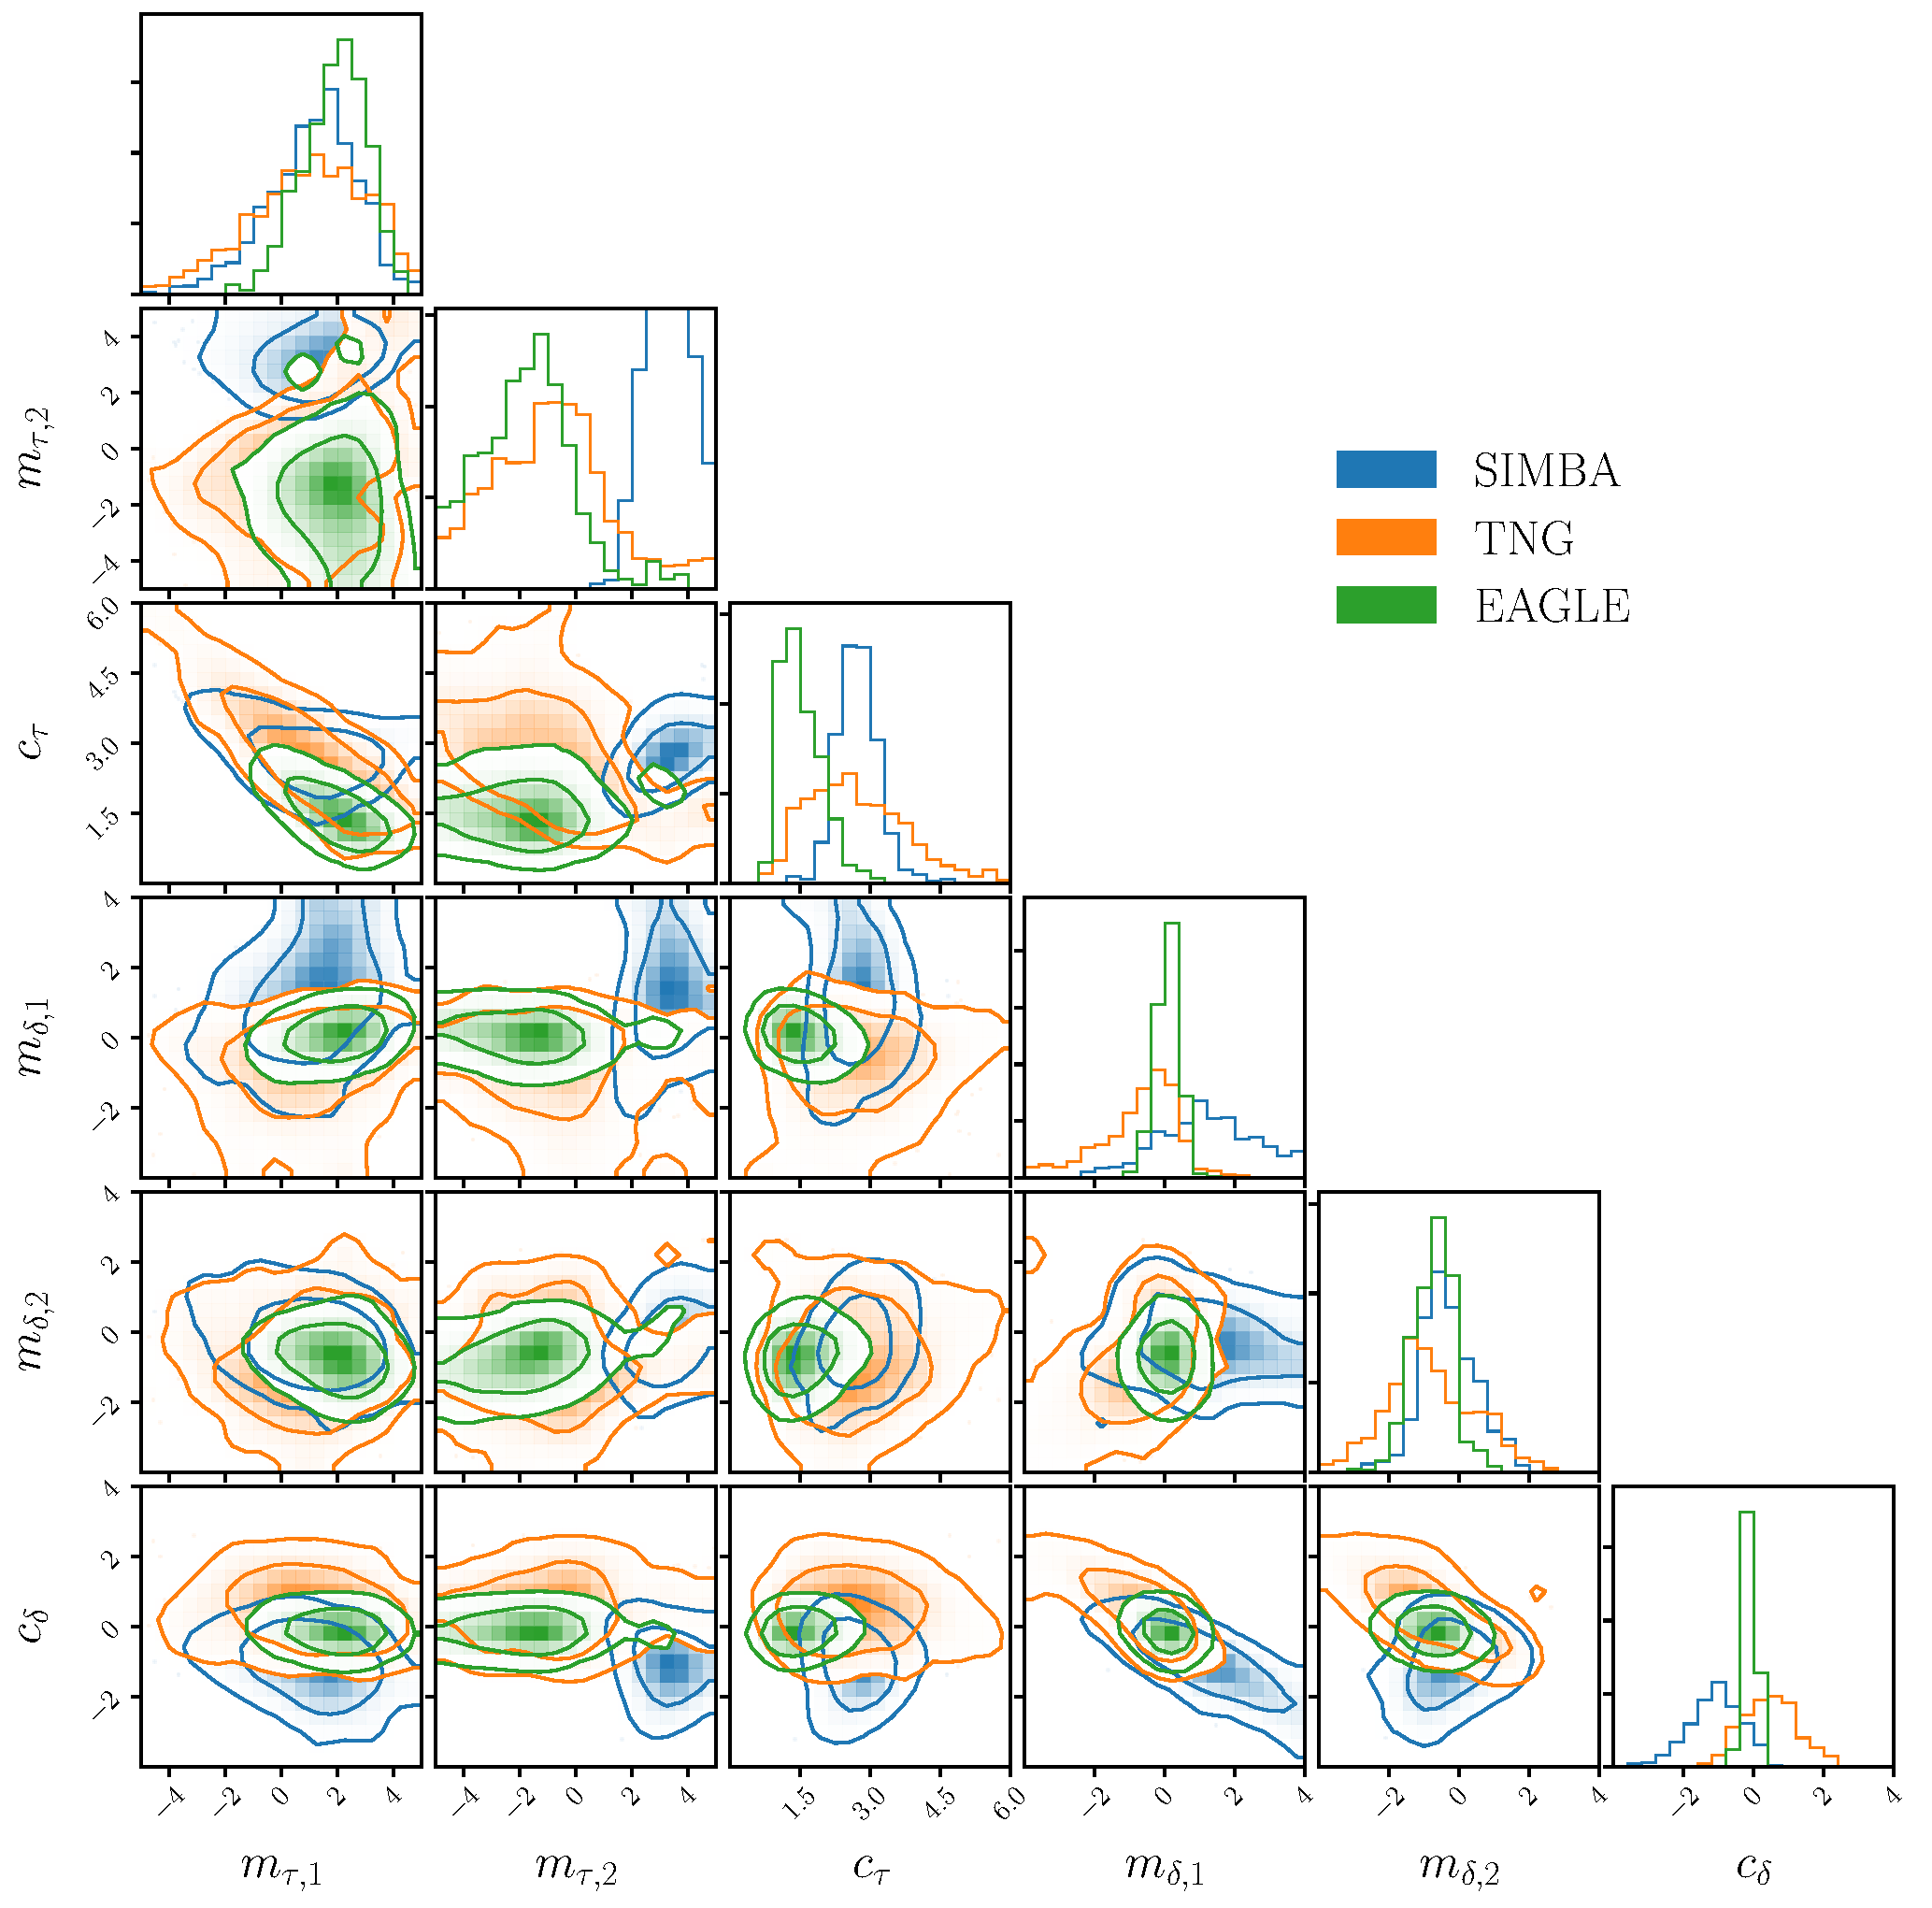
\includegraphics[width=\textwidth]{figs/abc.pdf}
    \caption{\label{fig:abc}
    Posterior distributions of DEM parameters for the SIMBA (orange), TNG
    (blue), and EAGLE (green) hydrodynamical simulations. The contours mark the $68\%$
    and $95\%$ confidence intervals. The posteriors are derived using
    Approximate Bayesian Computation with Population Monte Carlo
    (Section~\ref{sec:abc}). We focus on the DEM posteriors for TNG and EAGLE
    since SIMBA requires dust attenuation to reverse the relationship between
    color and $\sfr$ in order to account for it overpredicting low mass starburst 
    galaxies. Based on the posteriors, we find that \emph{galaxies with higher
    $M_*$ have overall higher dust attenuation and galaxies with lower $\sfr$
    have overall higher dust attenuation.}
    }
\end{center}
\end{figure}
